\documentclass{beamer}
\usepackage[T1]{fontenc}
\usepackage{textcomp}
\usepackage[utf8x]{inputenc}
\usepackage[danish]{babel}
\usepackage[garamond]{mathdesign}
\usepackage{url}
\usepackage{listings}
\usepackage{graphicx}
\usepackage{soul}

\renewcommand{\ttdefault}{pcr} % bedre typewriter font
\renewcommand{\rmdefault}{ugm} % garamond
\renewcommand{\sfdefault}{phv} % sans-serif font

\title{Fladuino}
\subtitle{Funktionel reaktiv programmering på indlejrede enheder}

\author{Martin Dybdal \and Troels Henriksen \and Jesper Reenberg}

\institute{\textrm{Datalogisk Institut, Københavns Universitet}}
\date{\today}

\mode<presentation>
{
  \usetheme{Frankfurt}
  %\usetheme{Warsaw} 
  \definecolor{uofsgreen}{rgb}{.125,.5,.25}
  \definecolor{natvidgreen}{rgb}{.196,.364,.239}
  \definecolor{kugrey}{rgb}{.4,.4,.4}
  \usecolortheme[named=uofsgreen]{structure}
  \usefonttheme[onlylarge]{structuresmallcapsserif}
  \usefonttheme[onlysmall]{structurebold}
}

\logo{
\includegraphics[height=1.5cm]{../diku.png}}

\usenavigationsymbolstemplate{} % fjern navigation

\lstset{language     = Haskell,
        extendedchars= true,
        breaklines   = false,
        tabsize      = 2,
        showstringspaces = false,
        basicstyle   = \small\ttfamily,
        commentstyle = \em,
        inputencoding= utf8
      }

\setcounter{tocdepth}{1}

\begin{document}

\frame{\titlepage}


\section{Flask}
\subsection{Flask}
\begin{frame}[t]
  \frametitle{Flask} 
  \framesubtitle{Dataflow-baseret reaktivt programmingssprog
    til sensor netværk.}

  \begin{block}{Reaktivitet}
    Et reaktivt system adskiller sig ved at det skal behandle værdier
    der varierer kontinuerligt. For eksempel aflæsninger fra en
    sensor.
  \end{block}

  \pause
  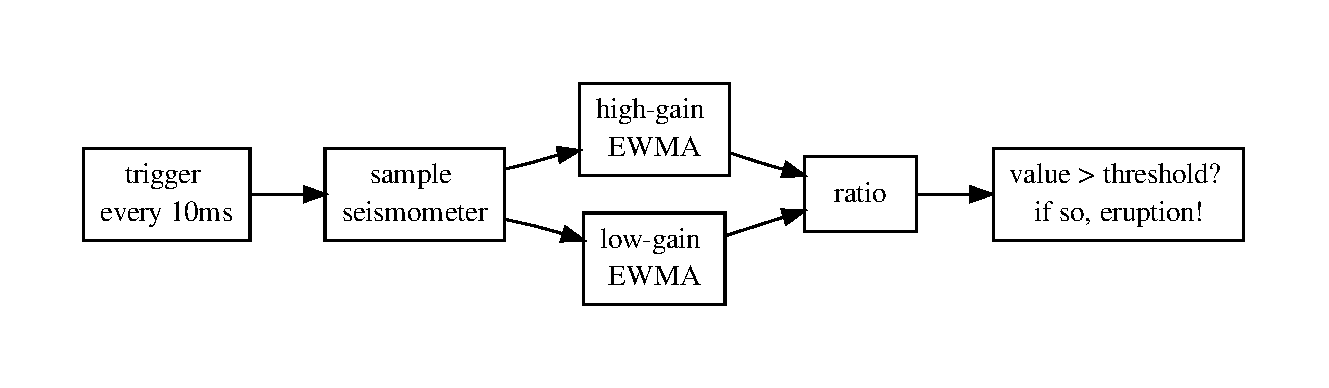
\includegraphics[width=\textwidth]{flask-ewma}

  \pause
  Statisk ikke dynamisk dataflow.

  Atomiske delgrafer
 
\end{frame}

\begin{frame}[t, fragile]
  \frametitle{Eksempelprogram} 

  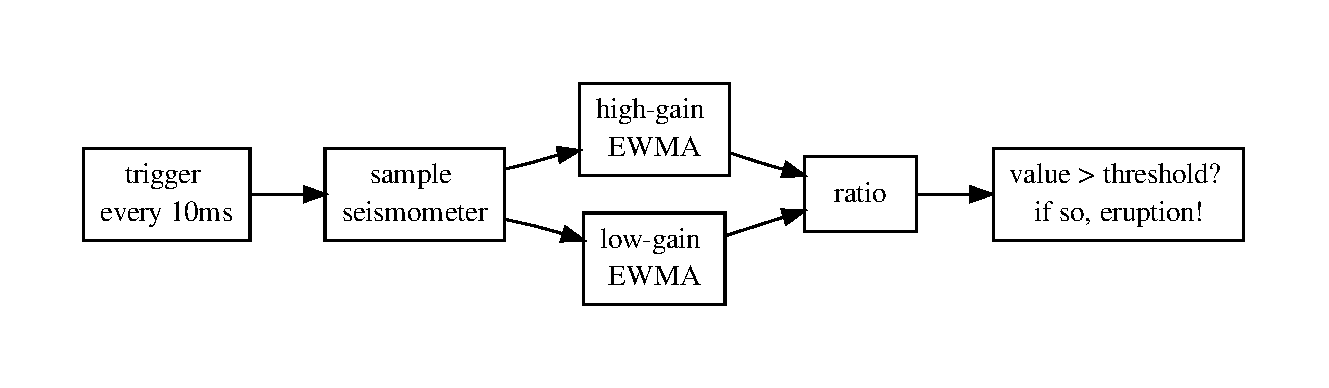
\includegraphics[width=\textwidth]{flask-ewma}
  \pause
\tiny

\begin{verbatim}
ewma :: Double -> S Double -> S Double
ewma gain = sintegrate zero
               [$exp| \(x, xold) ->
                        let x = $flo:gain * x +
                                (1.0 - $flo:gain) * xold
                        in (x, x) |]
    where
      zero :: N Double
      zero = liftN [$exp| 0.0 |]
\end{verbatim}

\pause
\normalsize
\begin{itemize}
\item 
  Haskell: metasprog
\item 
  Red og NesC: objektsprog (via quasiquotations)
\item 
  \verb|sintegrate| er en \textit{streamoperator}
\end{itemize}

\end{frame}


\begin{frame}[t, fragile]
  \frametitle{Et kig på Flask-typer}
Eksemplet fra før:
  \tiny
\begin{verbatim}
ewma :: Double -> S Double -> S Double
ewma gain = sintegrate zero
               [$exp| \(x, xold) ->
                        let x = $flo:gain * x +
                                (1.0 - $flo:gain) * xold
                        in (x, x) |]
    where
      zero :: N Double
      zero = liftN [$exp| 0.0 |]
\end{verbatim}
\normalsize
\pause

Stream operatoren \verb|sintegrate|:
\tiny
\begin{verbatim}
sintegrate  ::  forall a b c eta . (Reify a, Reify b, Reify c,
                                    LiftN eta ((a, c) -> (b, c)))
            =>  N c
            ->  eta
            ->  S a
            ->  S b
\end{verbatim}
\normalsize

\pause
Flytte typer og værdier til ``node-level'':

\begin{itemize}
\item Medlemmer af \verb|Reify| er Haskell-typer der har en ækvivalent
  type på ``node-level'' (her Red). 
\pause
\item \verb|LiftN eta a| angiver at \textit{værdien} eta, har en
  repræsentation \\ på ``node-level'' (dvs. værdier vi kan generere
  C-kode ud fra).
\end{itemize}

\end{frame}


\section{Oversættelsesstrategi}
\subsection{Flask $\rightarrow$ Sensornetværkskode}
\begin{frame}[t]
  \frametitle{Oversættelsesstrategi} 
  \framesubtitle{Flask $\rightarrow$ Sensornetværkskode}

  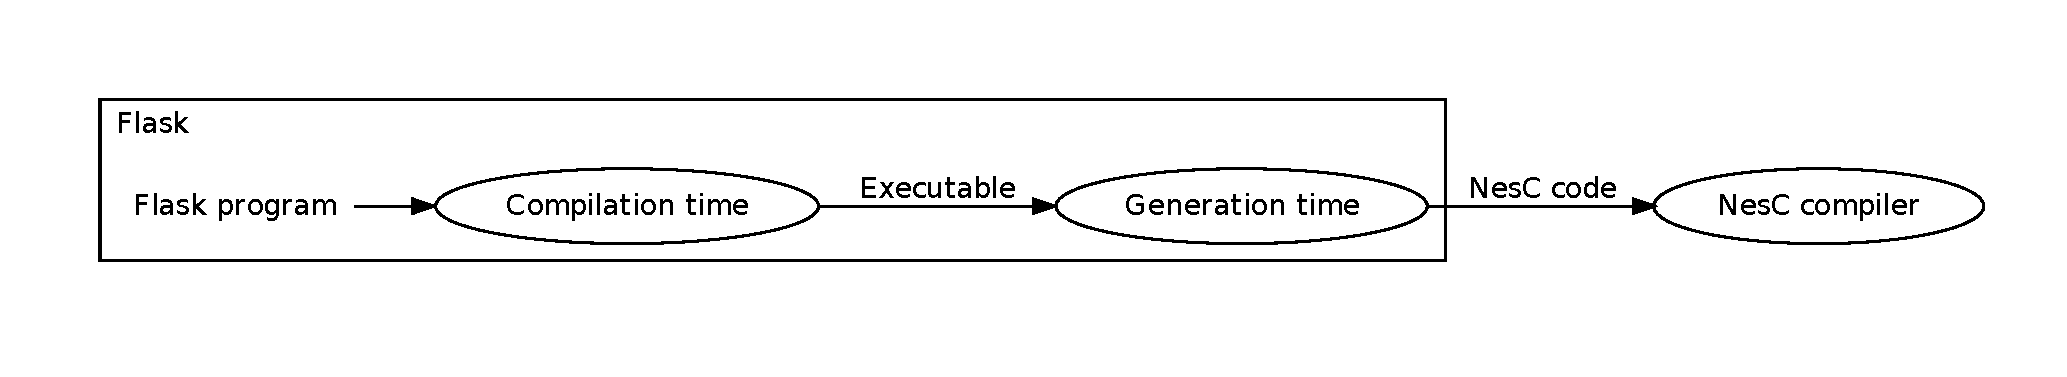
\includegraphics[width=\textwidth]{flask-simple}

\begin{description}
  \item[Compile time] Som det første parses indholdet af eventuelle
    quasiquotations og det resulterende syntaks træ indsættes på deres
    pladser (med huller). Generator programmet typetjekkes og
    compiles af GHC.
\item[Generation time] 
  Det resulterende program køres og genererer så NesC kode --- et
  sensornetværksprog.

\item[Maskinkode]
  NesC koden kan så oversættes til maskinekode af en NesC oversætter.   
\end{description}
\end{frame}

\subsection{Kodegenerering}
\begin{frame}[t]
  \frametitle{Oversættelsesstrategi} 
  \framesubtitle{Kodegenerering}

  \begin{itemize}
  \item Haskell-repræsentationen af en dataflow graf, evaluerer til en
    repræsentation af knuder (stream-operatorer) og kanter.
  \item For hver operator $o$ genereres en $o\_in$ og en $o\_out$
    funktion. (I nogle tilfælde er flere $o\_in$ funktioner
    nødvendige.)
  \end{itemize}

  

\end{frame}


\end{document}
